    \item The solution to the system of equations
          \[
              \myvec{2 & 5\\-4 & 3}\myvec{x\\y}=\myvec{2\\-30}
          \]
          is
	  \hfill(ME 2016)
	  )
          \begin{enumerate}
              \begin{multicols}{4}
                  \item $6, 2$
                  \item $-6, 2$
                  \item $-6, -2$
                  \item $6, -2$
              \end{multicols}
          \end{enumerate}
  \item A rigid ball of weight 100 N is suspended with the help of a string. The ball is pulled by a horizontal force $\vec{F}$ such that the string makes an angle of $30\degree$ with the vertical. The magnitude of force $\vec{F}$ (in N) is \rule{1cm}{0.01pt}.
	  \hfill(ME 2016)
          \begin{figure}[H]
              \centering
              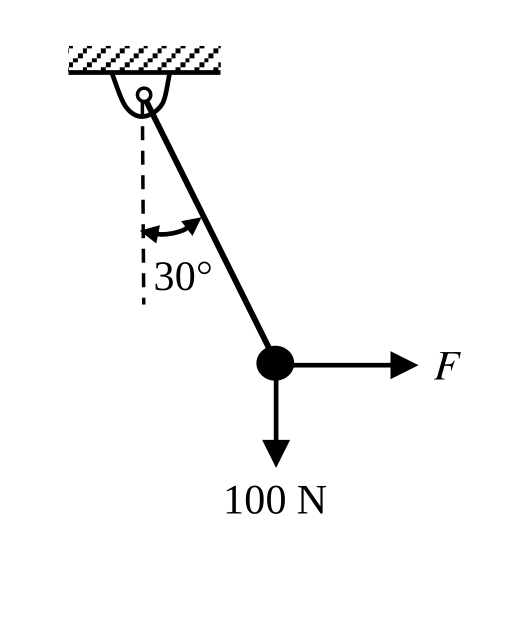
\includegraphics[scale=0.3]{GATE/2016/ME/figs/q6.png}
              \caption{}
              \label{q6}
          \end{figure}
    \item Gauss-Seidel method is used to solve the following equations (as per the given order):
          \begin{align}
              x_1 + 4x_2 + 8x_3 & = 12 \\
              2x_1 + x_2 + x_3  & = 5  \\
              x_1 + x_2 + x_3   & = 6
          \end{align}
          Assuming initial guess as $x_1 = x_2 = x_3 = 0$, the value of $x_2$ after the first iteration is \rule{1cm}{0.01pt}.
	  \hfill(ME 2016)
    \item A block of mass $m$ rests on an inclined plane and is attached by a string to the wall as shown in the figure. The coefficient of static friction between the plane and the block is 0.25. The string can withstand a maximum force of 20 N. The maximum value of the mass (m) for which the string will not break and the block will be in static equilibrium is \rule{1cm}{0.01pt} kg.
          Take $\cos \theta = 0.8$ and $\sin \theta = 0.6$.
          Acceleration due to gravity $g = 10$ m/s$^2$.
	  \hfill(ME 2016)
          \begin{figure}[H]
              \centering
              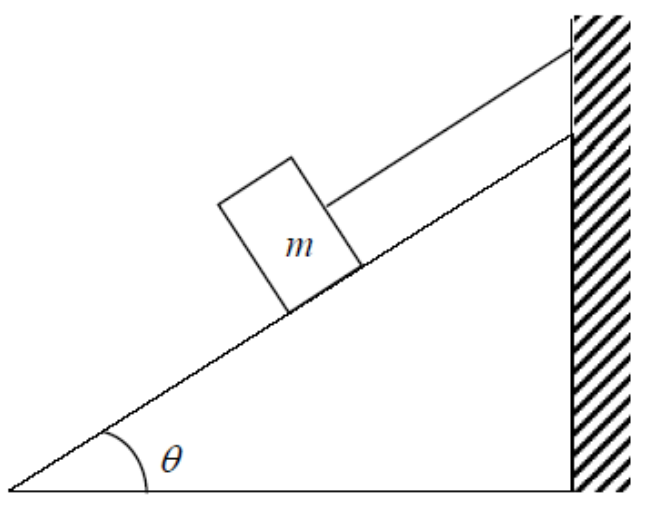
\includegraphics[scale=0.3]{GATE/2016/ME/figs/q30}
              \caption{}
              \label{q30}
          \end{figure}
    \item Consider a triangle $PQR$ with initial coordinates of the vertices as $\vec{P}$(1,3), $\vec{Q}$(4,5) and $\vec{R}$(5,3.5). The triangle is rotated in the X-Y plane about the vertex $\vec{P}$ by angle $\theta$ in clockwise direction. If $\sin \theta = 0.6$ and $\cos \theta = 0.8$, the new coordinates of the vertex $\vec{Q}$ are

	  \hfill(ME 2016)
          \begin{enumerate}
              \begin{multicols}{4}

                  \item (4.6, 2.8)

                  \item (3.2, 4.6)

                  \item (7.9, 5.5)

                  \item (5.5, 7.9)

              \end{multicols}

          \end{enumerate}
